\documentclass{beamer}

\usetheme[]{Rochester}
\usecolortheme{beaver}
\usepackage[latin1]{inputenc}
\usepackage{graphics}

\author{Will Webberley}
\date{Autumn 2014}
\institute[COMSC]{Cardiff School of Computer Science and Informatics}



\title{The `Physical' Interface: Software}
\subtitle{CM2101: Human-Computer Interaction}

\begin{document}

\frame{\titlepage}

\frame{
    \frametitle{Software interface}
    \begin{itemize}
        \item Link between the hardware interface and application logic in an electronic system
        \item Forms a layer of abstraction between the user's cognitive model and the system model
        \item Part of the gulfs of execution and evaluation
        \item Used for input (\alert{execution}) and output (\alert{evaluation})
    \end{itemize}
}

\frame{
    \frametitle{Software interface}
    \begin{center}
        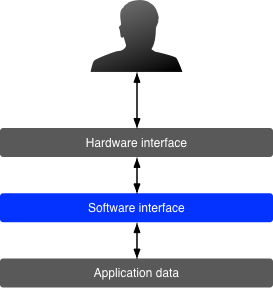
\includegraphics[width=6cm]{media/software_interface.png}
    \end{center}
}

\frame{
    \frametitle{Software interface}
    \begin{itemize}
        \item Must always be manipulated through the \alert{hardware layer}
        \item Interaction with the software interface directly manipulates memory
        \item Multiple types
        \begin{itemize}
            \item Text-only interface (e.g. console, single-user)
            \item Limitied graphical interface (usually single-input e.g. `old' TVs, boilers)
            \item Graphical user interface
        \end{itemize}
    \end{itemize}
}

\frame{
    \frametitle{Graphical user interface}
    \begin{itemize}
        \item Contains the controls to manipulate data and memory
        \item Contains the controls to run programs and processes
        \item Provides ability to navigate (e.g. scroll, change view)
        \item Provides containers (e.g. a window) to host an program-specific UI
        \item Provides decorators and surrounding context to windows
        \item Rendered in a hardware \alert{display}
        \item Requires some form of \alert{graphics processing} (e.g. a GPU)
    \end{itemize}
}

\frame{
    \frametitle{GUI types: Activity-, screen-, navigation-based}
    \begin{columns}
        \column{.5\textwidth}    
            Examples 
            \begin{itemize}
                \item iOS, Android, WP8
            \end{itemize}
        \column{.5\textwidth}
            Features
            \begin{itemize}
                \item (Multi-)touch, screen is input+output, modal
            \end{itemize}
    \end{columns}
    \vskip10pt
    \begin{center}
        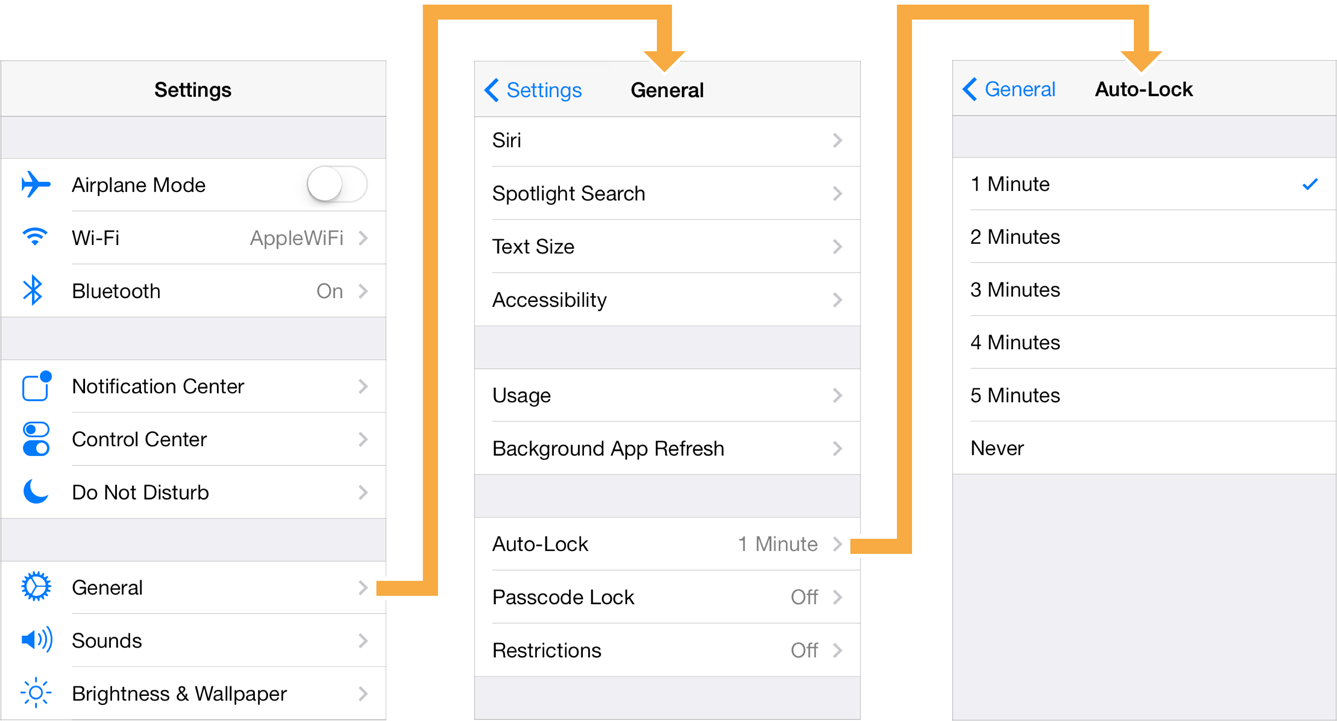
\includegraphics[width=11cm]{media/navigation.png}
    \end{center}
}

\frame{
    \frametitle{GUI types: OS-restricted-windowed interfaces}
    \begin{columns}
        \column{.5\textwidth}
            Examples
            \begin{itemize}
                \item in OS X, Windows
            \end{itemize}
            Features
            \begin{itemize}
                \item Traditionally `floating'
                \item Touch or keyboard+mouse
                \item Limited configurability
                \item More freedom than in mobile devices
                \item More input hardware devices typically available than in mobile devices
            \end{itemize}
        \column{.6\textwidth}
            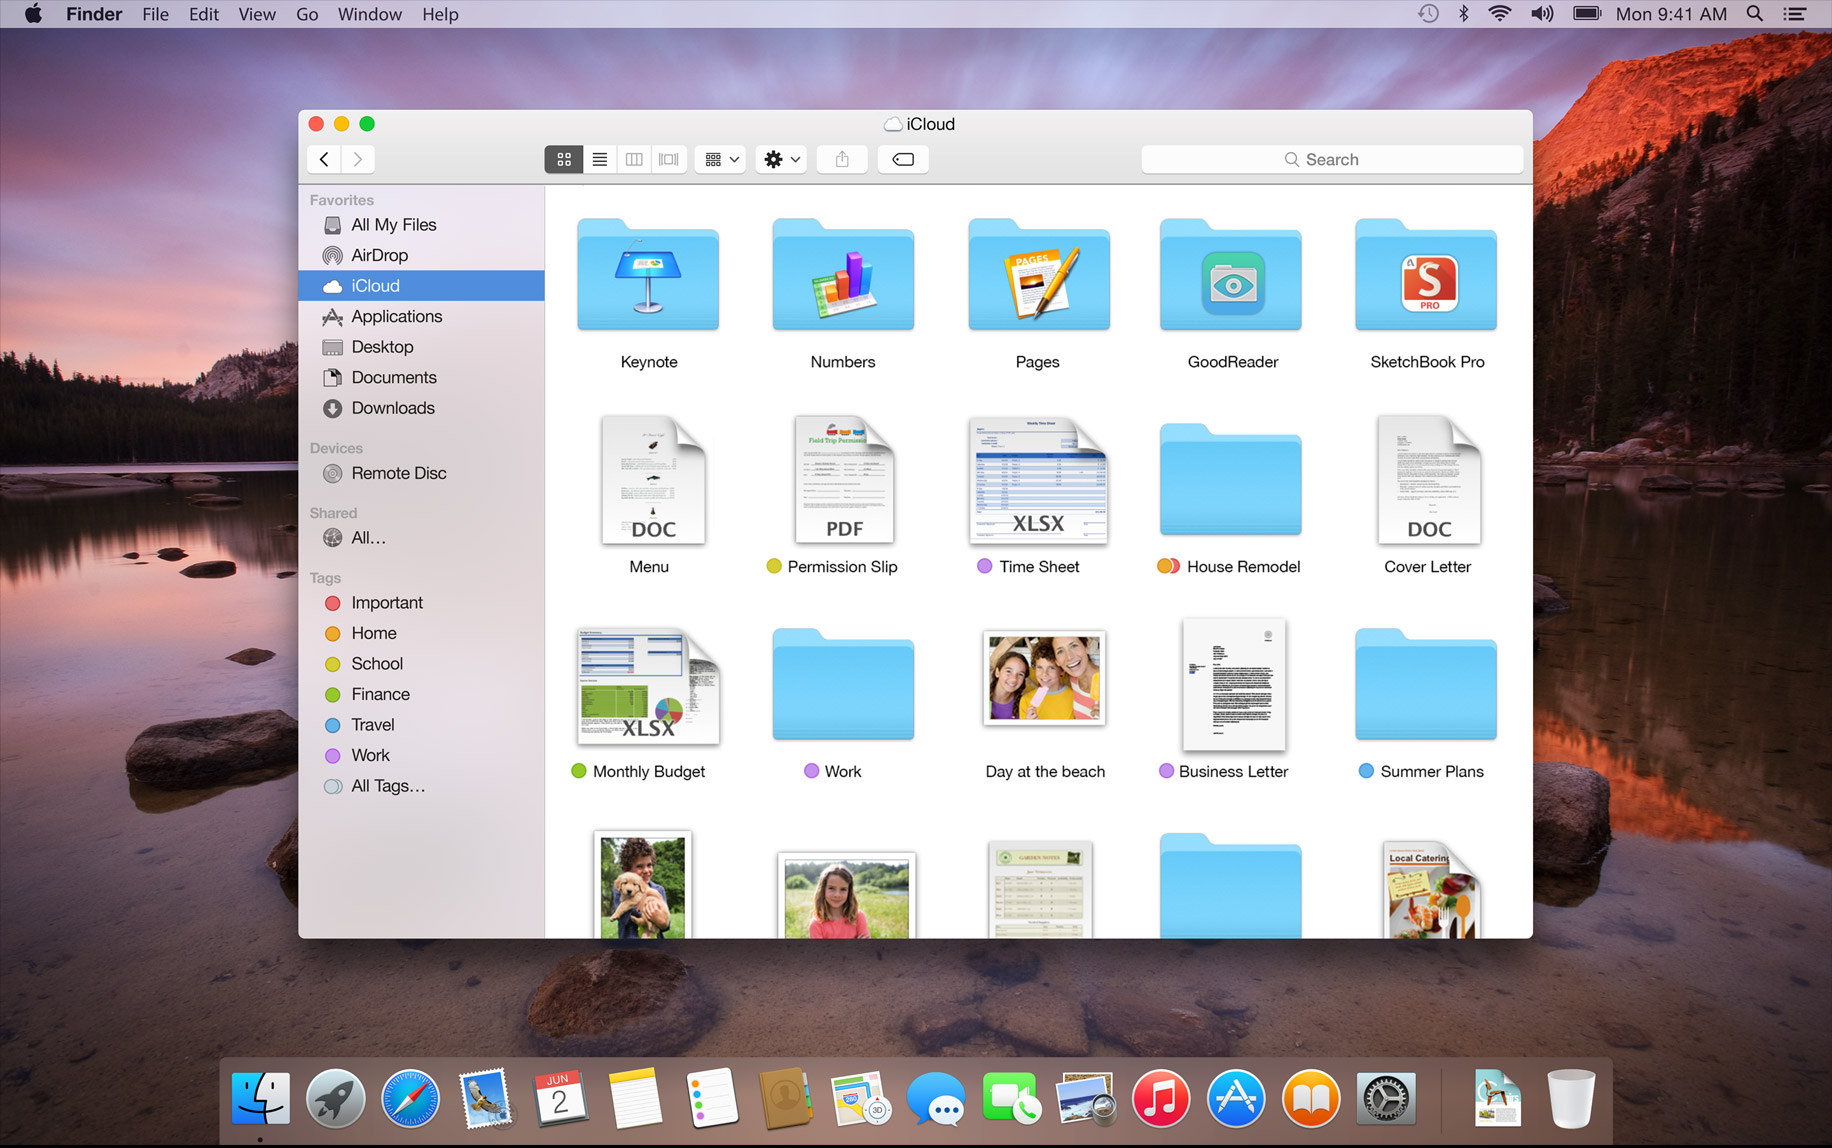
\includegraphics[width=6cm]{media/yosemite.jpg}
    \end{columns}
}

\frame{
    \frametitle{GUI types: Other floating window managers}
    \begin{columns}
        \column{.5\textwidth}
            Examples
            \begin{itemize}
                \item XFCE, GNOME, twm, fluxbox
                \item Many 1000s designed for the X11 or Wayland window systems 
                \item Some more feature rich (known as \alert{Desktop Environments})
            \end{itemize}
            Features
            \begin{itemize}
                \item Touch or keyboard+mouse
                \item More highly configurable
                \item + benefits from OS-restricted interfaces
            \end{itemize}
        \column{.6\textwidth}
            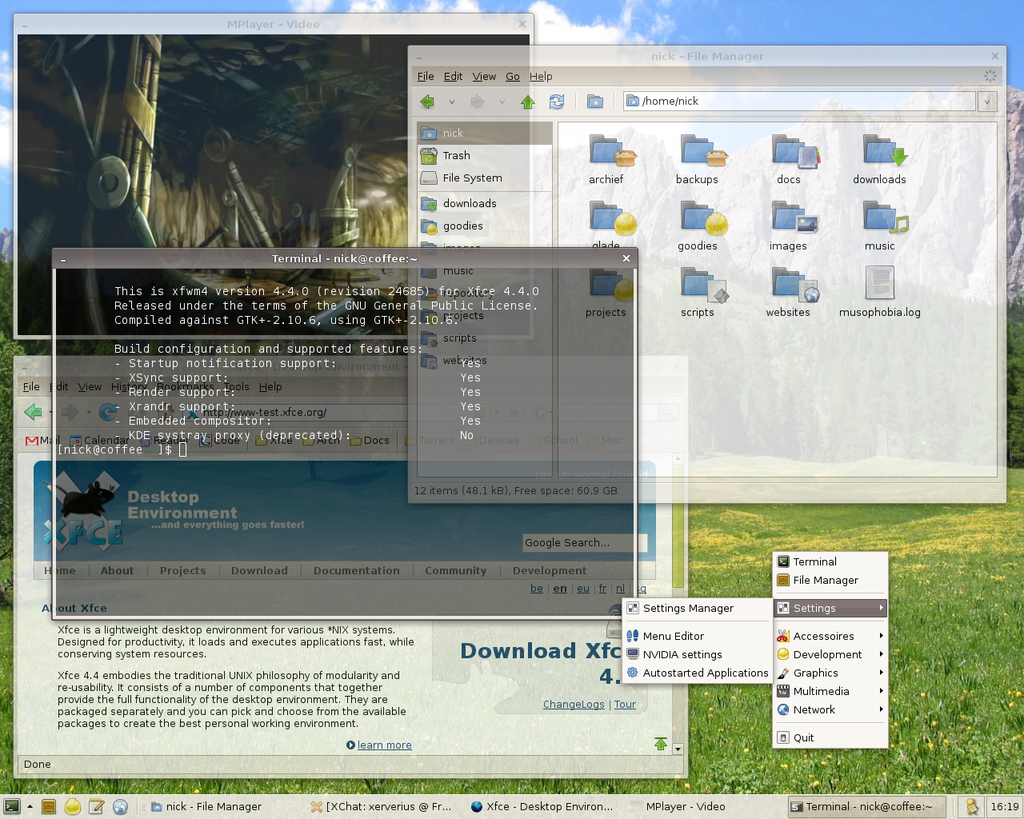
\includegraphics[width=6cm]{media/xfce.png}
    \end{columns}
}

\frame{
    \frametitle{GUI types: Tiled window managers}
    \begin{columns}
        \column{.5\textwidth}
            Examples
            \begin{itemize}
                \item awesomeWM, i3, dwm, xmonad 
                \item Many designed for the X11 or Wayland window systems 
                \item Addons available for systems like Windows to `emulate' tiling
            \end{itemize}
            Features
            \begin{itemize}
                \item Often keyboard-only (mouse control for GUI windows)
                \item Highly configurable
                \item Efficient and productive
            \end{itemize}
        \column{.6\textwidth}
            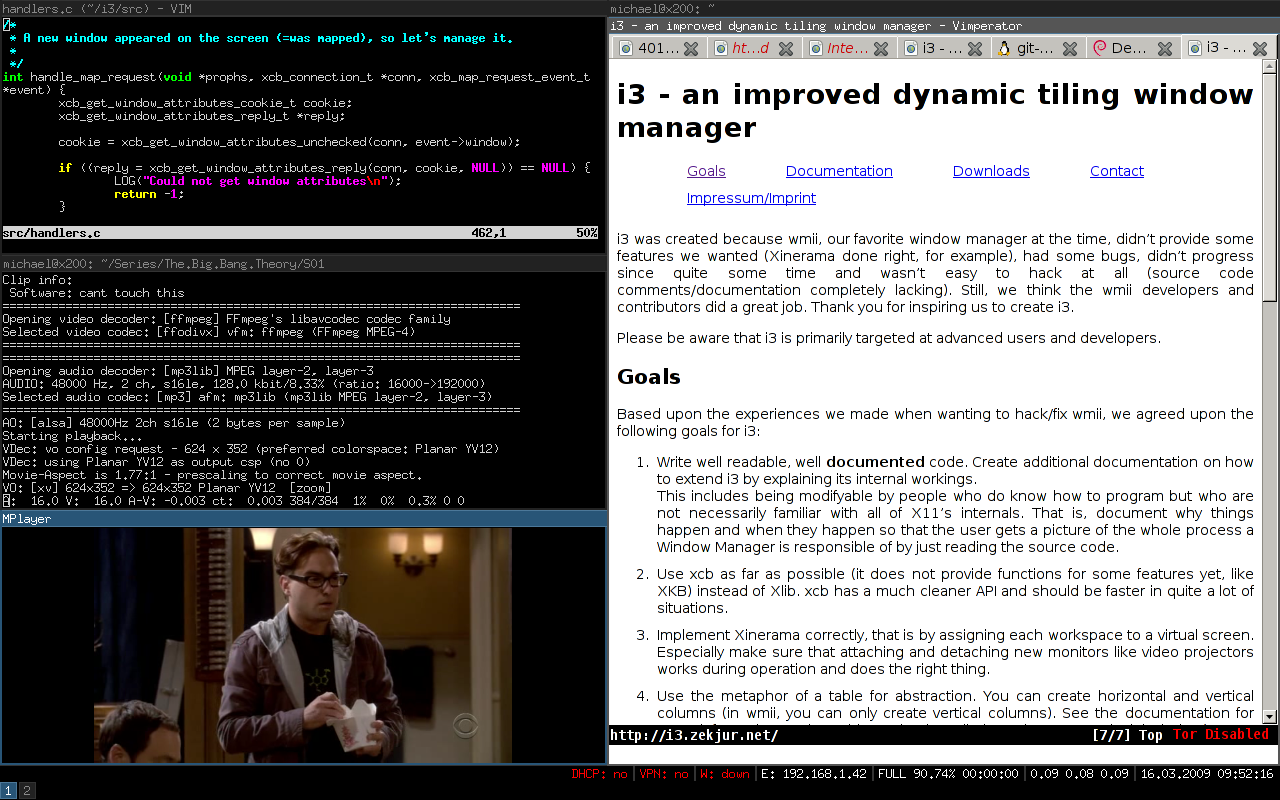
\includegraphics[width=6cm]{media/i3.png}
    \end{columns}
}

\frame{
    \frametitle{Software UI controls}
    \begin{itemize}
        \item Hosted inside a GUI
        \item Allows for \alert{modifying} and \alert{viewing} memory structures
        \item Can be datatype specific, e.g.:
        \begin{itemize}
            \item Checkbox: binary
            \item Radio: multi-dimensional nominal (e.g. array)
            \item Textbox: string/int/etc.
        \end{itemize}
        \item Useful for entering or viewing data in different ways
        \item Designers should use the components most appropriate for both inputting and outputting data
        \item Again, these controls are manipulated through \alert{hardware interfaces}
    \end{itemize}   
}

\frame{
    \frametitle{UI control examples: Button}
    \begin{center}
        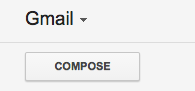
\includegraphics[width=4cm]{media/button.png}
    \end{center} 
    \alert{Uses}
    \begin{itemize}
        \item Binary input (e.g. `turned on' and `turned off')
        \item Repeated input (e.g. email compose button)
    \end{itemize}
    \vskip20pt
    \alert{Implementations (most major platforms)}
    \begin{itemize}\footnotesize
        \item Android - \texttt{button = new Button();}
        \item iOS - \texttt{button = UIButton.buttonWithType(UIButtonType.System)}
        \item HTML - \texttt{<button>Click me</button>}
    \end{itemize}
}

\frame{
    \frametitle{UI control examples: Checkbox}
    \begin{center}
        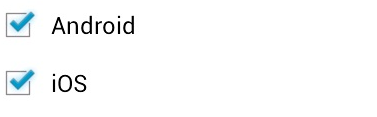
\includegraphics[width=4cm]{media/checkbox.png}
    \end{center} 
    \alert{Uses}
    \begin{itemize}
        \item One selection (`this thing' but not `those things')
        \item Some systems (e.g. iOS) use \alert{toggles} instead
        \item Some HTML `toggle' implementations have checkboxes underneath
    \end{itemize}
    \vskip20pt
    \alert{Implementations (most major platforms)}
    \begin{itemize}\footnotesize
        \item Android - \texttt{cb = new CheckBox();}
        \item HTML - \texttt{<input type="checkbox" />}
    \end{itemize}
}

\frame{
    \frametitle{UI control examples: Radio}
    \begin{center}
        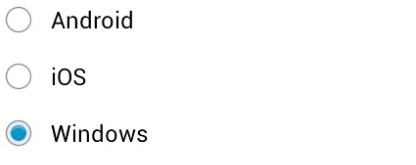
\includegraphics[width=4cm]{media/radio.png}
    \end{center} 
    \alert{Uses}
    \begin{itemize}
        \item Multiple-selection (`these things' but not `those things')
        \item Radio buttons are \alert{grouped} to constrain selection
        \item Some systems (e.g. iOS) use toggles instead
    \end{itemize}
    \vskip20pt
    \alert{Implementations (most major platforms)}
    \begin{itemize}\footnotesize
        \item Android - \texttt{rb = new RadioButton();}
        \item HTML - \texttt{<input type="radio" name="group\_name" />}
        \item iOS - use \texttt{UISegmentedControl}
    \end{itemize}
}

\frame{
    \frametitle{UI control examples: Textfield}
    \alert{Uses}
    \begin{itemize}
        \item Can be customised for different purposes:
        \begin{itemize}
            \item Text (incl. length, allowed characters)
            \item Number (incl. incrementer, constraints on decimal places)
            \item Email (automatically show `@' on mobile keyboards)
            \item Search
            \item Password (hide/obfuscate input characters)
            \item Longer text entry (e.g. textareas)
        \end{itemize}
        \item Many platforms \alert{decorate} fields differently depending on its purpose
        \item Placeholders allow for input \alert{suggestions}
    \end{itemize}
    \vskip5pt
    \alert{Implementations (most major platforms)}
    \begin{itemize}\footnotesize
        \item Android - \texttt{tv = new TextView();}
        \item HTML - \texttt{<input type="text|password|email|search|number" />}
        \item iOS - \texttt{tf: UITextField = UITextField()} 
    \end{itemize}
}

\frame{
    \frametitle{UI modal components}
    \begin{itemize}
        \item Usually temporarily appears above the rest of the UI
        \item Useful for prompting the user for action
        \item Prevents modification of underlying UI until action is finished
    \end{itemize}
}

\frame{
    \frametitle{UI modal component examples: Dialog boxes}
    \begin{columns}
        \column{.5\textwidth}
            \begin{itemize}
                \item Prompt user for input or action
                \item Display alerts or errors
                \item Indicate long-running tasks
                \item Display contextual information
            \end{itemize}
        \column{.5\textwidth}
            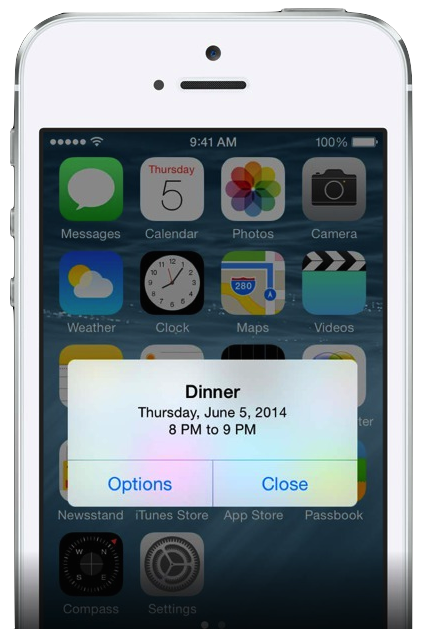
\includegraphics[width=4cm]{media/dialog.png}
    \end{columns}
}

\frame{
    \frametitle{UI modal component examples: Menus}
    \begin{columns}
        \column{.5\textwidth}
            \begin{itemize}
                \item Tidy up UI by placing some actions in menus
                \item \alert{Context} menus for specific objects (e.g. press and hold a Tweet)
            \end{itemize}
        \column{.5\textwidth}
            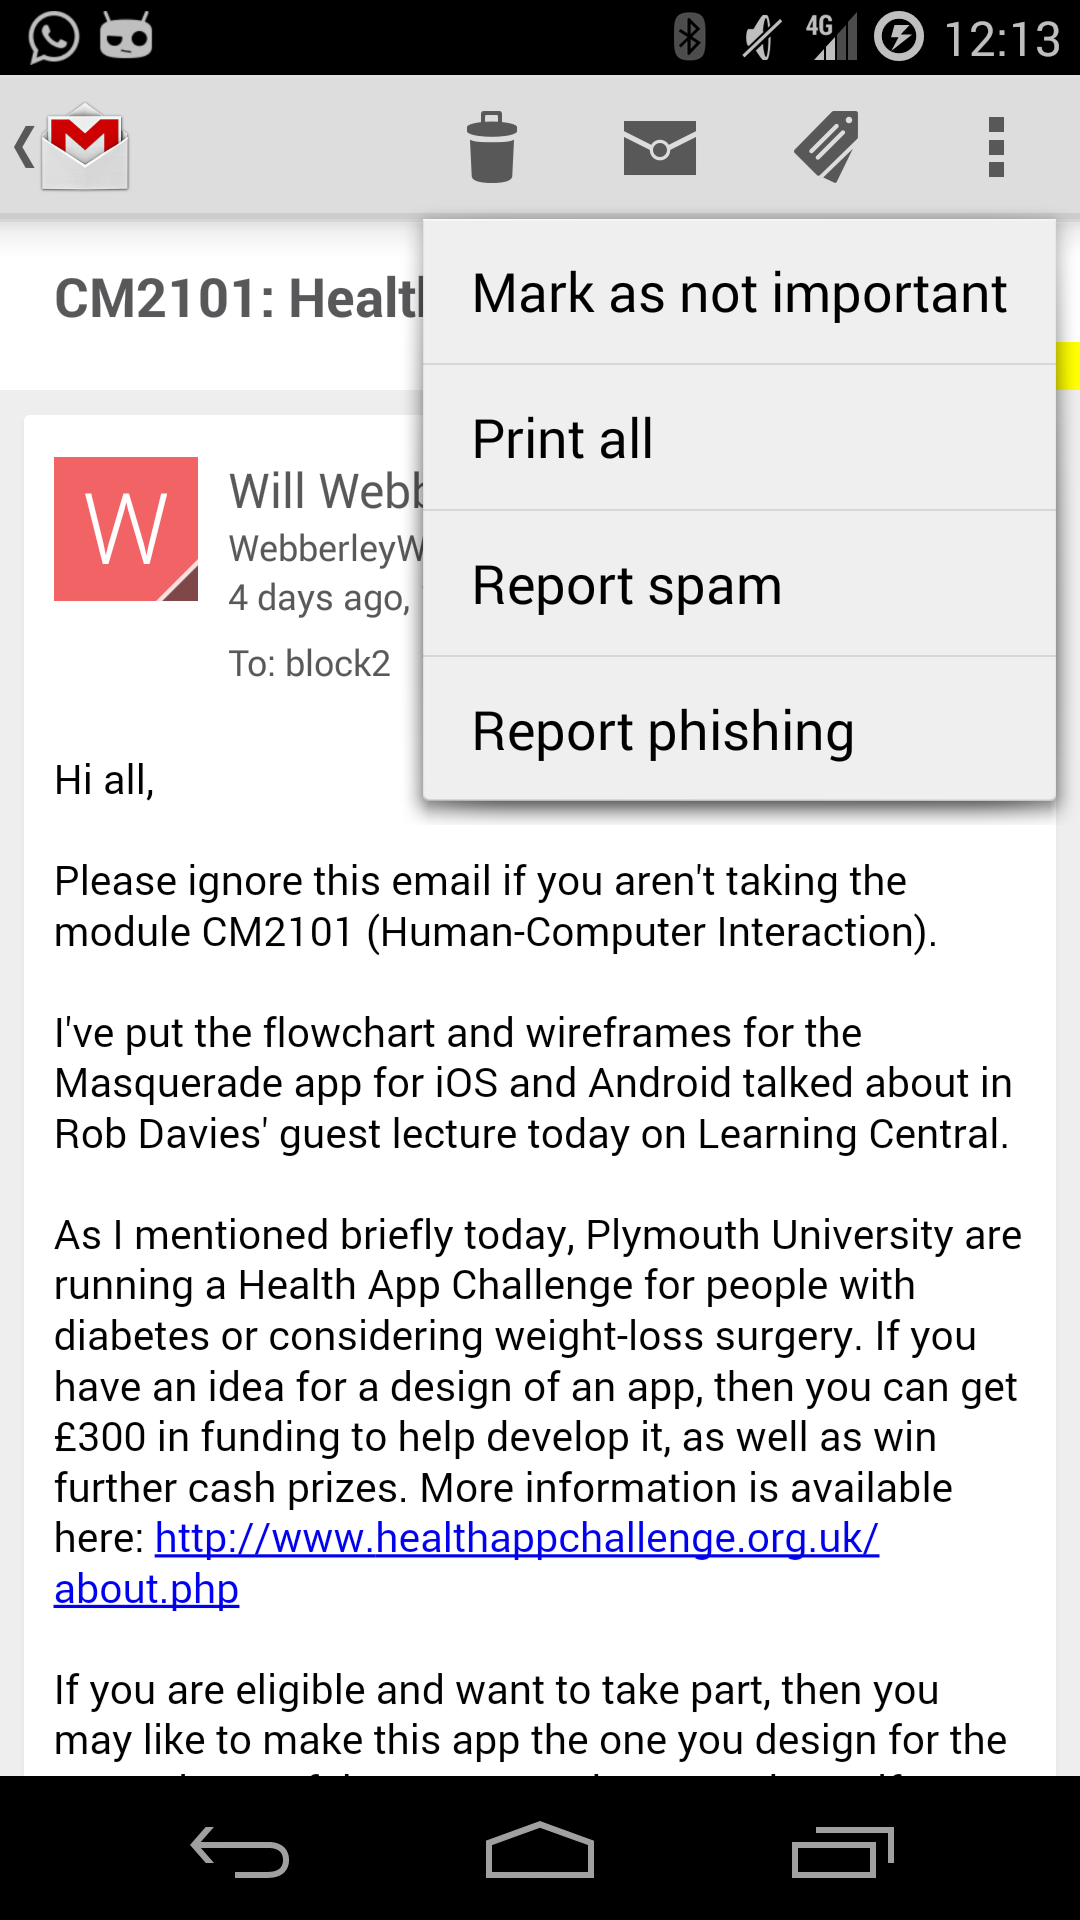
\includegraphics[width=4cm]{media/menu.png}
    \end{columns}
}

\frame{
    \frametitle{UI navigation structures}
    \begin{itemize}
        \item Allow for navigation within a screen or window
        \item Typically contain UI controls/components
        \item Group relevant UI components together
        \item Useful for `extending' the UI beyond the dimensions of the physical screen
    \end{itemize}
}

\frame{
    \frametitle{UI navigation structure examples: Scroll views}
    \begin{columns}
        \column{.5\textwidth}
            \begin{itemize}
                \item Place content within a scrolling view to navigate \textit{widhin} the view
                \item Useful for overflow of content
                \item Horizontal and vertical scrolling (e.g. maps or zoomed-in images)
            \end{itemize}       
        \column{.5\textwidth}
            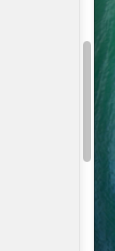
\includegraphics[width=3cm]{media/scroll.png}
    \end{columns}
}

\frame{
    \frametitle{UI navigation structure examples: Tabbed views}
    \begin{columns}
        \column{.5\textwidth}
            \begin{itemize}
                \item Logically partition the UI
                \item Able to quickly switch (or swipe) between tabs
                \item Can see current information in the scope of the rest of the screen
            \end{itemize}       
        \column{.5\textwidth}
            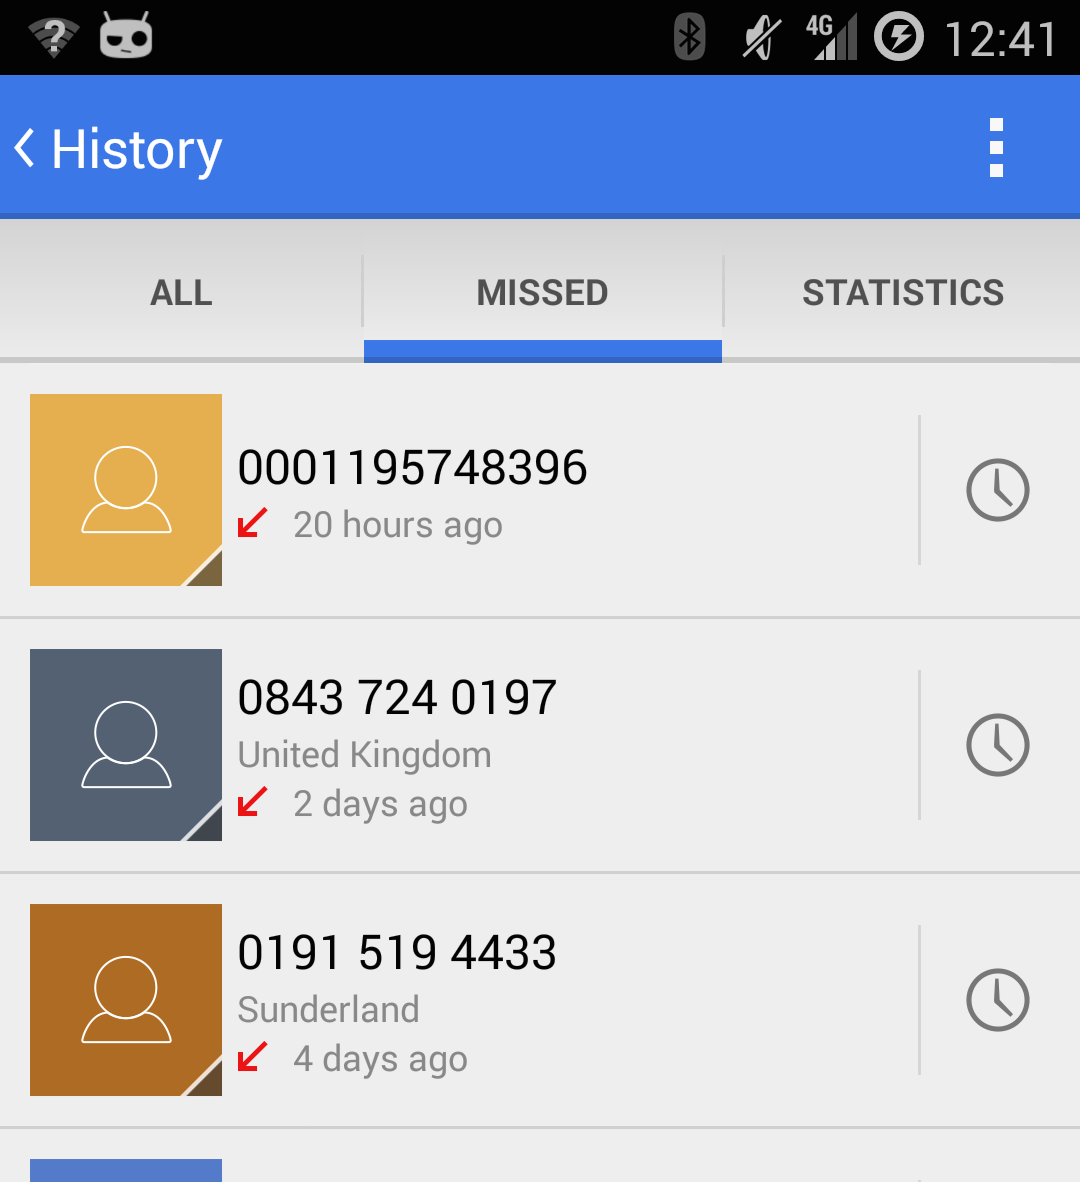
\includegraphics[width=4cm]{media/tabbed.png}
    \end{columns}
}

\frame{
    \frametitle{UI navigation structure examples: Refresher}
    \begin{columns}
        \column{.5\textwidth}
            \begin{itemize}
                \item `Pull to refresh'
                \item Load more info to UI (from server or storage)
                \item Should retrieve the \alert{latest information}
                \item Appropriate for time-ordered interfaces
            \end{itemize}       
        \column{.5\textwidth}
            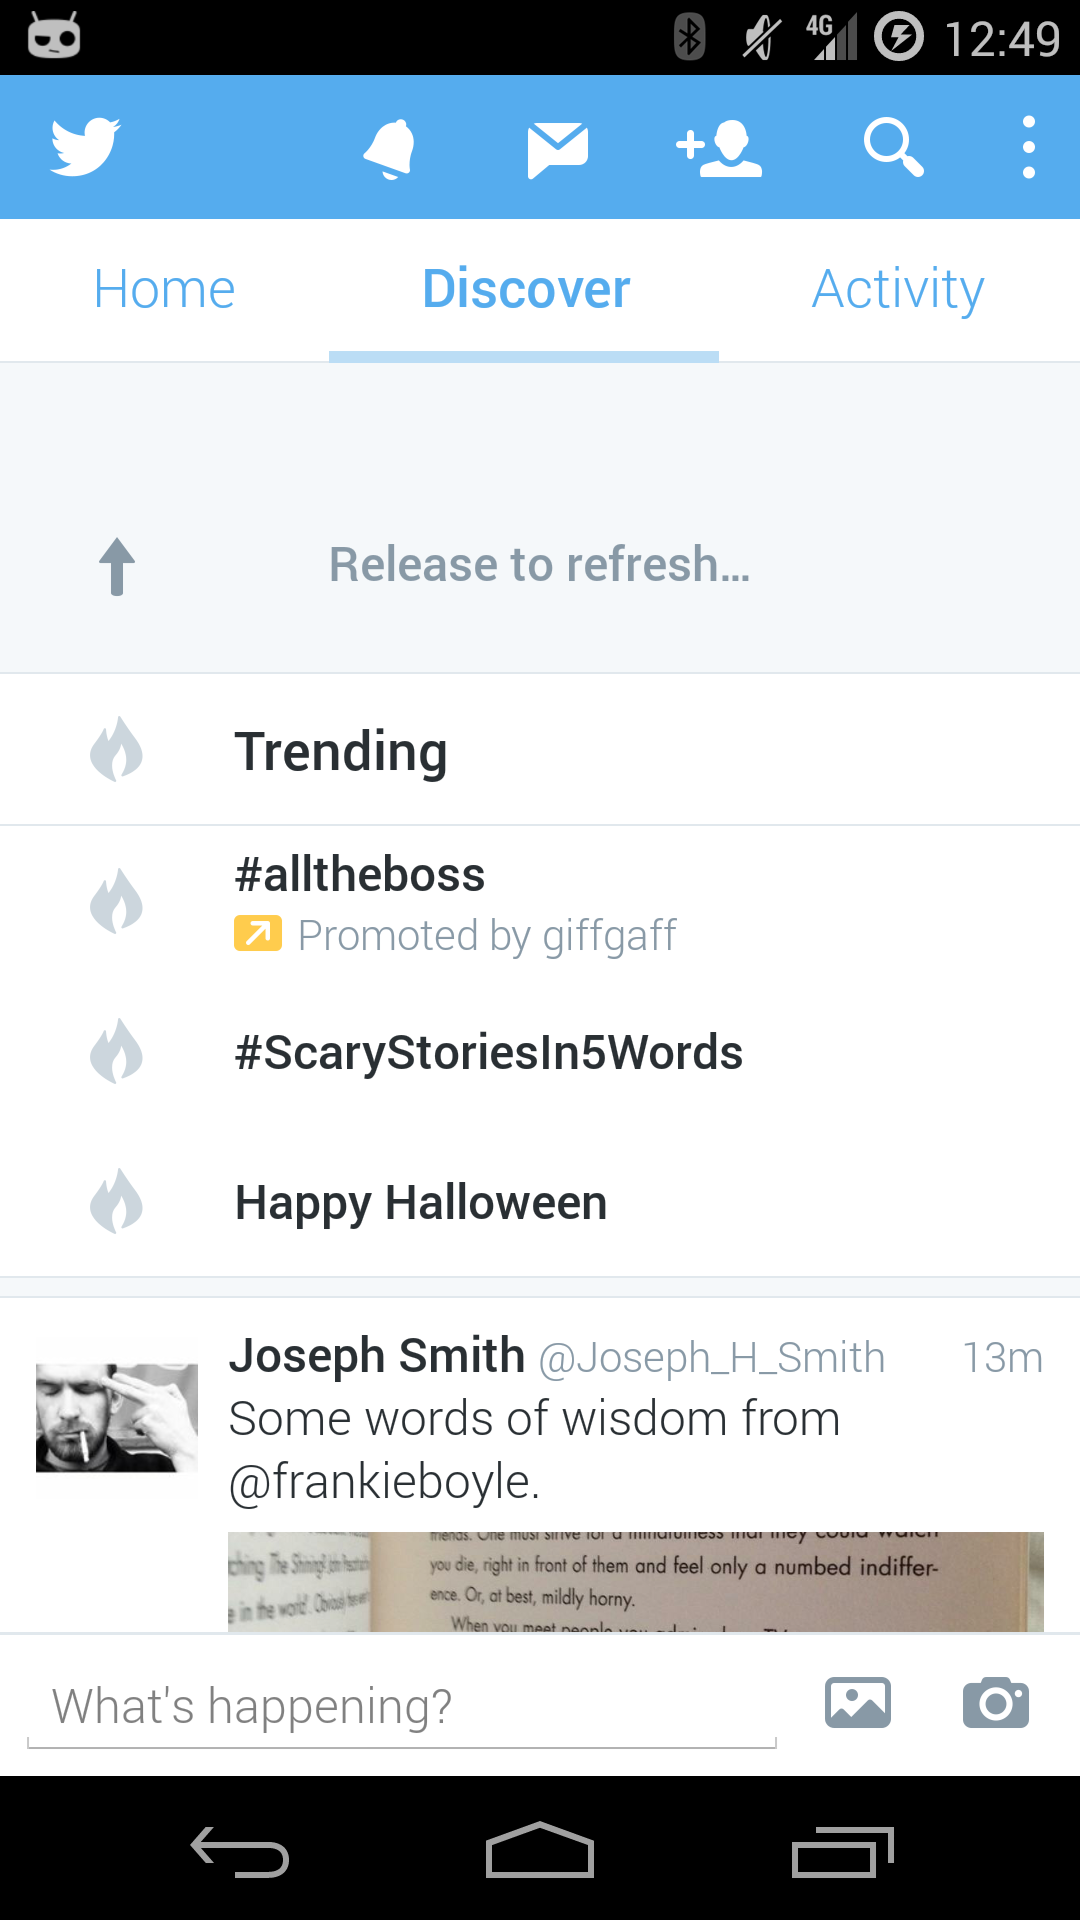
\includegraphics[width=4cm]{media/pull_refresh.png}
    \end{columns}
}

\frame{
    \frametitle{UI navigation structure examples: Infinite scroll}
    \begin{columns}
        \column{.5\textwidth}
            \begin{itemize}
                \item Opposite of \textit{Refresher}
                \item Load more info to UI (from server or storage)
                \item Should retrieve \alert{older information}
                \item Appropriate for time-ordered interfaces
            \end{itemize}       
        \column{.5\textwidth}
            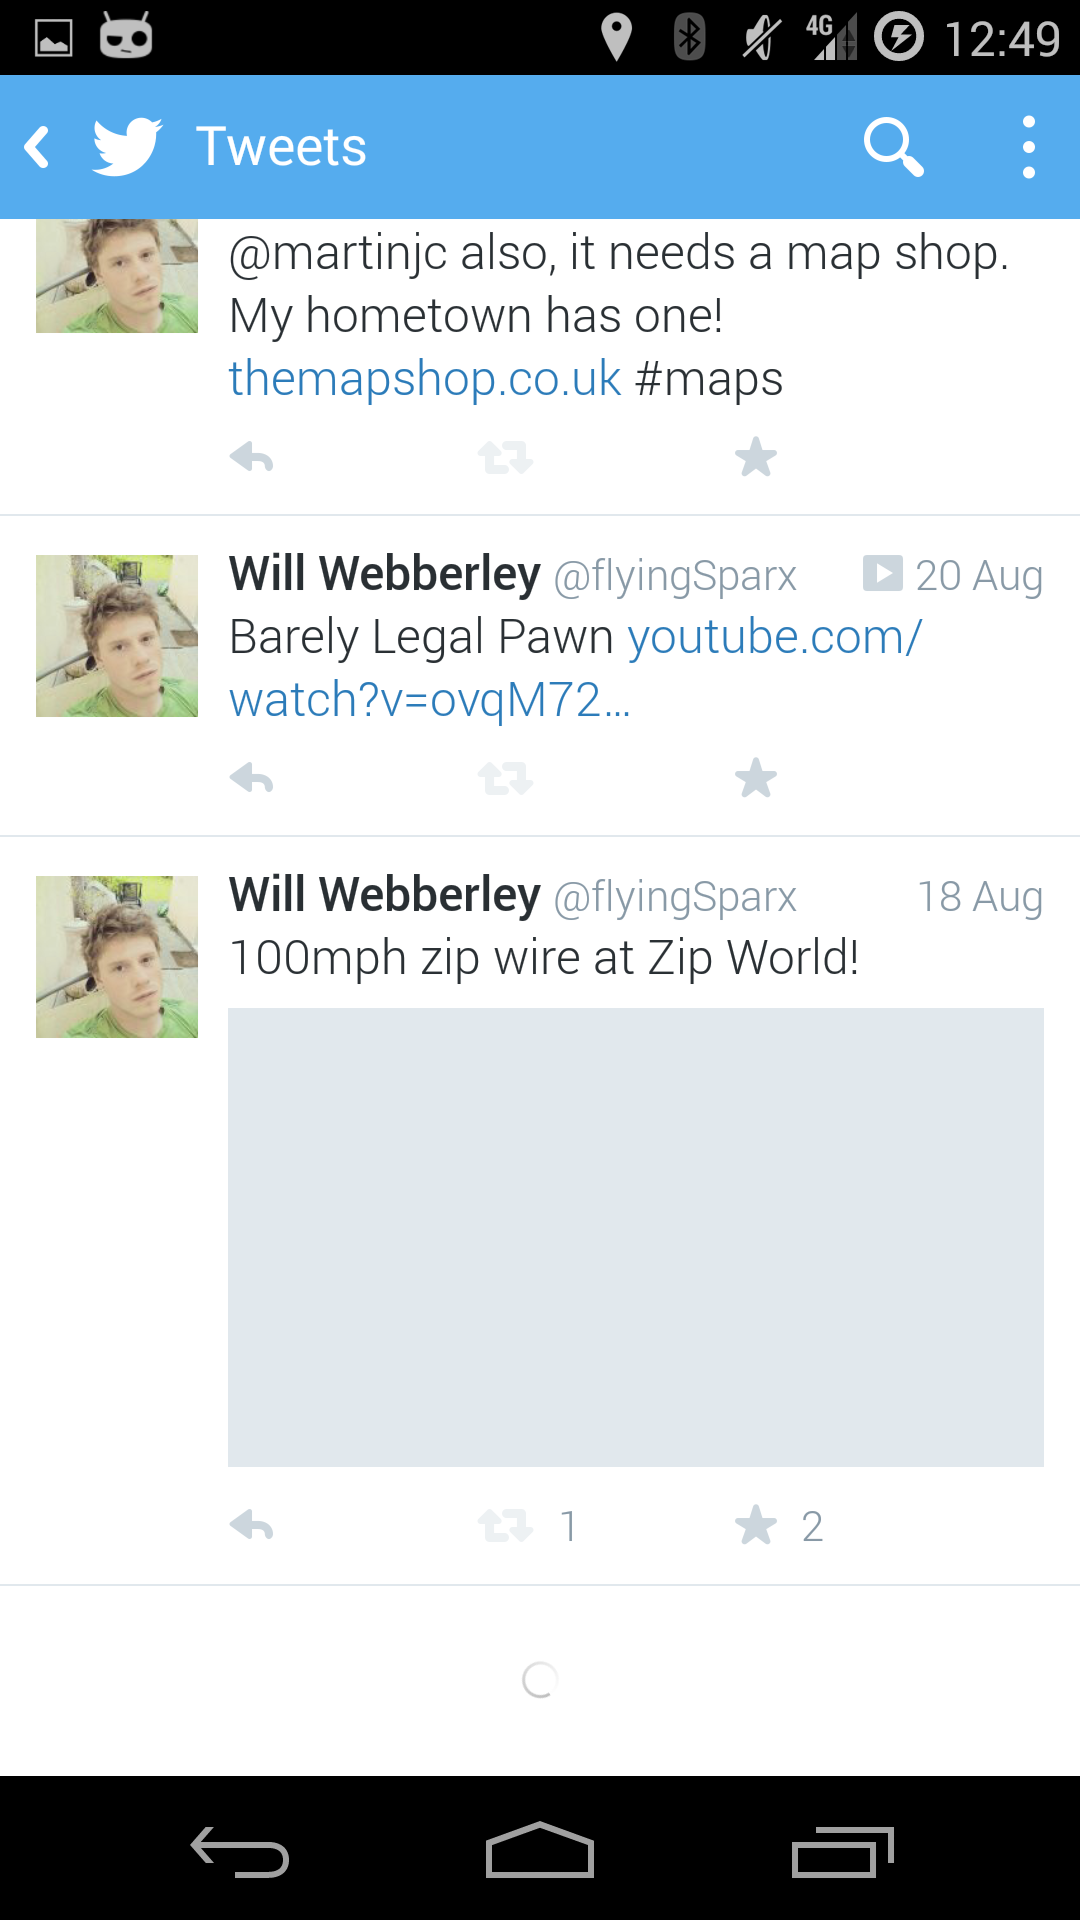
\includegraphics[width=4cm]{media/infinite_scroll.png}
    \end{columns}
}

\frame{
    \frametitle{UI components in general}
    \begin{itemize}
        \item Many more than described earlier
        \item Easy to customise for own use (e.g. checkbox $\rightarrow$ toggle)
        \item Easy to extend
        \item Choose the right components (you don't need to use \textit{all})
        \item Remember: designs should largely be task-driven
    \end{itemize}
}   

\frame{
    \frametitle{Decorating components}
    \begin{columns}
        \column{.7\textwidth}
            \begin{itemize}    
                \item Associate icons with actions
                \item Apply \alert{cultural constraint}
                \item Invoke \alert{recognition} and \alert{familiarity}
                \item Decorate using
                \begin{itemize}
                    \item Colours
                    \item Icons (alone or with text)
                \end{itemize}
                \item Allows for \alert{branding} 
            \end{itemize}
        \column{.3\textwidth}   
            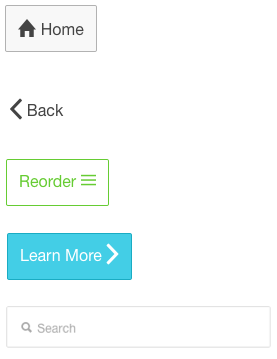
\includegraphics[width=5cm]{media/decoration.png}
    \end{columns}
}

\frame{
    \frametitle{Designing the software interface}
    \begin{itemize}
        \item Design to help improve learnability (and other usability principles)
        \item Design to facilitate data-input and do tasks (gulf of \alert{execution})
        \item Design to facilitate understanding of what the system is `saying' (gulf of \alert{evaluation})
        \item Ensure it can be manipulated given the hardware
    \end{itemize}
}   

\frame{
     \frametitle{Revision questions}
     \begin{enumerate}
        \item Explain how the software interface can be modified to help the gulf of evaluation?
        \item As well as full GUIs, what other types of software interfaces exist?
        \item Typically, what kind of hardware handles output of a software interface?
        \item What is a \textit{window} in a GUI?
        \item What is meant by the term \textit{tiling window manager}?
        \item Why are navigation-style interfaces useful on mobile devices?
        \item What is the difference between a checkbox and a radio button?
        \item Explain how modal interface components are useful.
        \item How might a designer allow for refreshing content in a time-based interface?
     \end{enumerate}
}

\frame{
    \frametitle{Summary}
    \begin{itemize}
        \item Context of software interfaces within a system
        \item Link between software and hardware
        \item Software interfaces and human cognition
        \item GUI types
        \item Software components
        \item Component decoration
    \end{itemize}
}    

\end{document}
